
\documentclass[border=10pt, 12pt]{standalone}
\usepackage[svgnames]{xcolor}
\usepackage{amsmath}
\usepackage{pgfplots}
\pgfplotsset{compat=newest}
\usepackage[sfdefault]{FiraSans}
\usepackage{FiraMono}
\renewcommand*\familydefault{\sfdefault}
\begin{document}
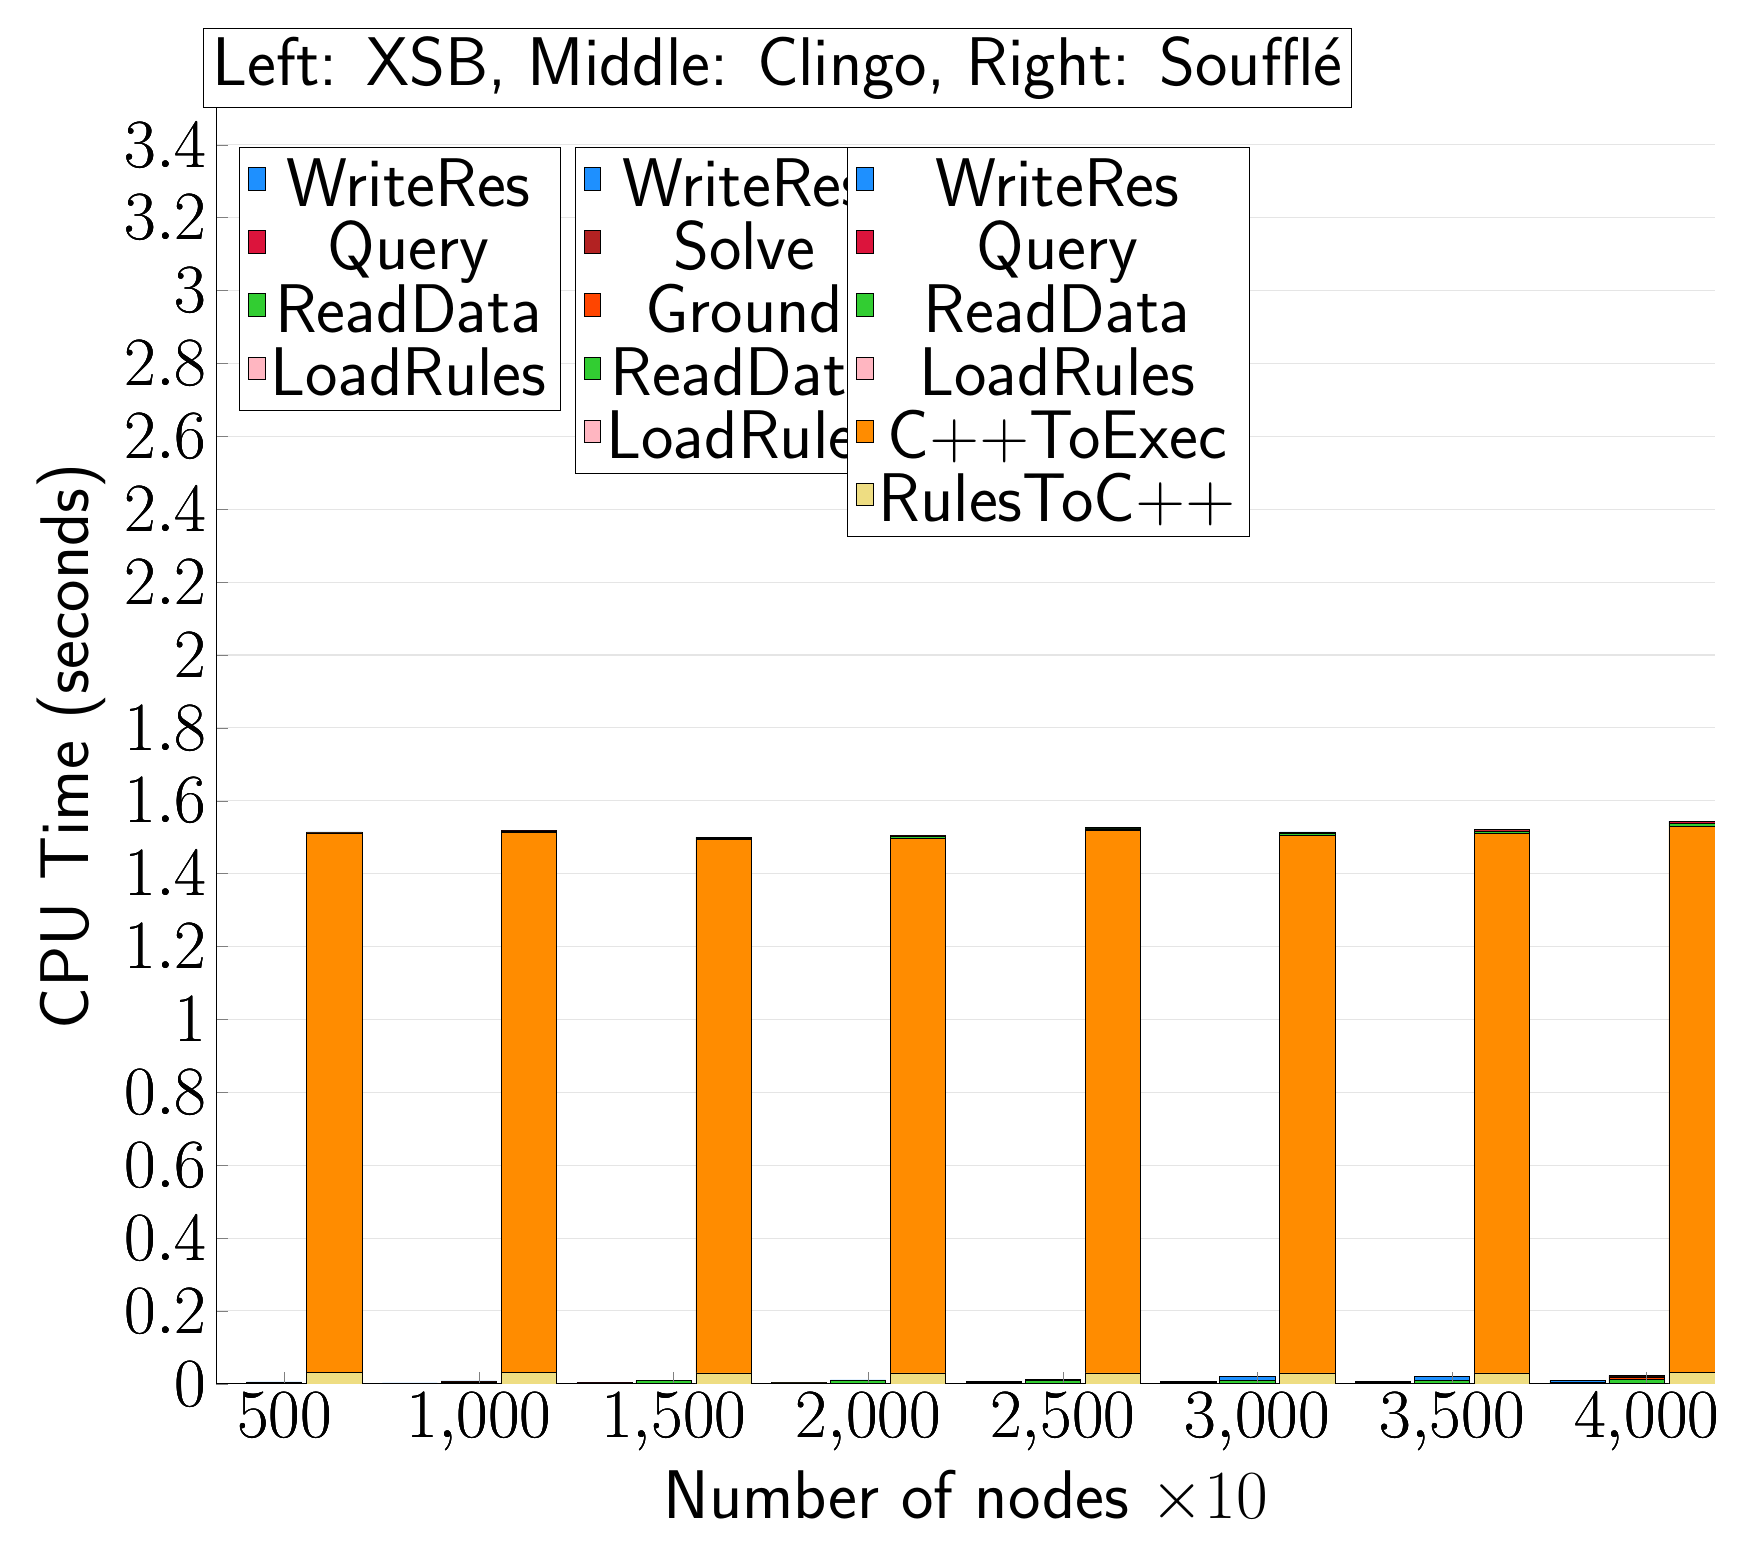
\begin{tikzpicture}
	\begin{axis}[bar shift=-25pt,
			ybar stacked,
			width=1.7\textwidth,
			bar width=0.7cm,
			ymajorgrids, tick align=inside,
			major grid style={draw=gray!20},
			xtick=data,
			ymin=0, ymax=3.5,
			axis x line*=bottom,
			axis y line*=left,
			enlarge x limits=0.05,
			legend style={
					at={(0.23, 0.97)},
					anchor=north east,
					legend columns=1,
					font=\Huge,
				},
			ylabel={CPU Time (seconds)},
			xlabel={Number of nodes $\times 10$},
			label style={font=\Huge},
			tick label style={font=\Huge},
		]
		\addlegendimage{fill=DodgerBlue, draw=black, line width=0.2pt}
		\addlegendentry{WriteRes}
		\addlegendimage{fill=Crimson, draw=black, line width=0.2pt}
		\addlegendentry{Query}
		\addlegendimage{fill=LimeGreen, draw=black, line width=0.2pt}
		\addlegendentry{ReadData}
		\addlegendimage{fill=LightPink, draw=black, line width=0.2pt}
		\addlegendentry{LoadRules}
		\addplot +[fill=LightPink, draw=black, line width=0.2pt] coordinates {
				(500, 0.0006251)
				(1000, 0.0006293999999999998)
				(1500, 0.0006049000000000003)
				(2000, 0.0006117000000000004)
				(2500, 0.0006043000000000005)
				(3000, 0.0006246000000000002)
				(3500, 0.0006211999999999998)
				(4000, 0.0006276999999999996)
			};
		\addplot +[fill=LimeGreen, draw=black, line width=0.2pt] coordinates {
				(500, 0.0005511999999999993)
				(1000, 0.0010302000000000002)
				(1500, 0.0014505)
				(2000, 0.0018939999999999999)
				(2500, 0.0023967)
				(3000, 0.0028251)
				(3500, 0.0032141)
				(4000, 0.0037044)
			};
		\addplot +[fill=Crimson, draw=black, line width=0.2pt] coordinates {
				(500, 7.300000000000047e-05)
				(1000, 0.0001425999999999994)
				(1500, 0.00020650000000000009)
				(2000, 0.0002692999999999994)
				(2500, 0.00035010000000000087)
				(3000, 0.0004404000000000008)
				(3500, 0.0005193999999999996)
				(4000, 0.0006082000000000004)
			};
		\addplot +[fill=DodgerBlue, draw=black, line width=0.2pt] coordinates {
				(500, 0.0005166999999999992)
				(1000, 0.0009725000000000008)
				(1500, 0.0014221999999999998)
				(2000, 0.0018493000000000006)
				(2500, 0.0023594999999999996)
				(3000, 0.0028949999999999996)
				(3500, 0.0033131000000000002)
				(4000, 0.003845)
			};
	\end{axis}

	\begin{axis}[bar shift=-3.7pt,
			ybar stacked,
			width=1.7\textwidth,
			bar width=0.7cm,
			ymajorgrids, tick align=inside,
			major grid style={draw=none},
			xtick=data,
			ymin=0, ymax=3.5,
			axis x line*=none,
			axis y line*=none,
			enlarge x limits=0.05,
			legend style={
					at={(0.454, 0.97)},
					anchor=north east,
					legend columns=1,
					font=\Huge,
				},
			label style={font=\Huge},
			tick label style={font=\Huge},
		]
		\addlegendimage{fill=DodgerBlue, draw=black, line width=0.2pt}
		\addlegendentry{WriteRes}
		\addlegendimage{fill=FireBrick, draw=black, line width=0.2pt}
		\addlegendentry{Solve}
		\addlegendimage{fill=OrangeRed, draw=black, line width=0.2pt}
		\addlegendentry{Ground}
		\addlegendimage{fill=LimeGreen, draw=black, line width=0.2pt}
		\addlegendentry{ReadData}
		\addlegendimage{fill=LightPink, draw=black, line width=0.2pt}
		\addlegendentry{LoadRules}
		\addplot +[fill=LightPink, draw=black, line width=0.2pt] coordinates {
				(500, 0.0)
				(1000, 0.0)
				(1500, 0.0)
				(2000, 0.0)
				(2500, 0.0)
				(3000, 0.0)
				(3500, 0.0)
				(4000, 0.0)
			};
		\addplot +[fill=LimeGreen, draw=black, line width=0.2pt] coordinates {
				(500, 0.0019999999999999996)
				(1000, 0.0029999999999999996)
				(1500, 0.008999999999999998)
				(2000, 0.008999999999999998)
				(2500, 0.009999999999999997)
				(3000, 0.009999999999999997)
				(3500, 0.009999999999999997)
				(4000, 0.011999999999999997)
			};
		\addplot +[fill=OrangeRed, draw=black, line width=0.2pt] coordinates {
				(500, 0.0009999999999999998)
				(1000, 0.0019999999999999996)
				(1500, 0.0)
				(2000, 0.0)
				(2500, 0.0)
				(3000, 0.0)
				(3500, 0.0)
				(4000, 0.007000000000000001)
			};
		\addplot +[fill=FireBrick, draw=black, line width=0.2pt] coordinates {
				(500, 0.0)
				(1000, 0.0009999999999999998)
				(1500, 0.0)
				(2000, 0.0)
				(2500, 0.0)
				(3000, 0.0)
				(3500, 0.0)
				(4000, 0.0010000000000000002)
			};
		\addplot +[fill=DodgerBlue, draw=black, line width=0.2pt] coordinates {
				(500, 0.0019999999999999996)
				(1000, 0.002)
				(1500, 0.0)
				(2000, 0.0020000000000000005)
				(2500, 0.0020000000000000005)
				(3000, 0.010000000000000004)
				(3500, 0.010000000000000004)
				(4000, 0.0030000000000000005)
			};
	\end{axis}

	\begin{axis}[bar shift=18pt,
			ybar stacked,
			width=1.7\textwidth,
			bar width=0.7cm,
			ymajorgrids, tick align=inside,
			major grid style={draw=none},
			xtick=data,
			ymin=0, ymax=3.5,
			axis x line*=none,
			axis y line*=none,
			enlarge x limits=0.05,
			legend style={
					at={(0.69, 0.97)},
					anchor=north east,
					legend columns=1,
					font=\Huge,
				},
			label style={font=\Huge},
			tick label style={font=\Huge},
		]
		\addlegendimage{fill=DodgerBlue, draw=black, line width=0.2pt}
		\addlegendentry{WriteRes}
		\addlegendimage{fill=Crimson, draw=black, line width=0.2pt}
		\addlegendentry{Query}
		\addlegendimage{fill=LimeGreen, draw=black, line width=0.2pt}
		\addlegendentry{ReadData}
		\addlegendimage{fill=LightPink, draw=black, line width=0.2pt}
		\addlegendentry{LoadRules}
		\addlegendimage{fill=DarkOrange, draw=black, line width=0.2pt}
		\addlegendentry{C++ToExec}
		\addlegendimage{fill=LightGoldenrod, draw=black, line width=0.2pt}
		\addlegendentry{RulesToC++}
		\addplot +[fill=LightGoldenrod, draw=black, line width=0.2pt] coordinates {
				(500, 0.031000000000000007)
				(1000, 0.031000000000000007)
				(1500, 0.030000000000000006)
				(2000, 0.030000000000000006)
				(2500, 0.030000000000000006)
				(3000, 0.030000000000000006)
				(3500, 0.030000000000000006)
				(4000, 0.031)
			};
		\addplot +[fill=DarkOrange, draw=black, line width=0.2pt] coordinates {
				(500, 1.4809999999999999)
				(1000, 1.483)
				(1500, 1.4640000000000002)
				(2000, 1.4669999999999999)
				(2500, 1.488)
				(3000, 1.475)
				(3500, 1.4800000000000002)
				(4000, 1.499)
			};
		\addplot +[fill=LightPink, draw=black, line width=0.2pt] coordinates {
				(500, 1.32e-05)
				(1000, 0.0)
				(1500, 0.0)
				(2000, 0.0)
				(2500, 0.0)
				(3000, 0.0)
				(3500, 1e-05)
				(4000, 0.0)
			};
		\addplot +[fill=LimeGreen, draw=black, line width=0.2pt] coordinates {
				(500, 0.0013585)
				(1000, 0.0023988000000000004)
				(1500, 0.0036106000000000007)
				(2000, 0.0046609)
				(2500, 0.0048955)
				(3000, 0.0057937)
				(3500, 0.007134800000000001)
				(4000, 0.008418100000000001)
			};
		\addplot +[fill=Crimson, draw=black, line width=0.2pt] coordinates {
				(500, 0.0005299)
				(1000, 0.0010607000000000001)
				(1500, 0.0015976)
				(2000, 0.0020704000000000005)
				(2500, 0.0022706)
				(3000, 0.0026808000000000005)
				(3500, 0.0033788)
				(4000, 0.0039652)
			};
		\addplot +[fill=DodgerBlue, draw=black, line width=0.2pt] coordinates {
				(500, 0.0004182)
				(1000, 0.0006336)
				(1500, 0.0008641999999999999)
				(2000, 0.0010643999999999999)
				(2500, 0.0011023)
				(3000, 0.0012483)
				(3500, 0.0015306999999999999)
				(4000, 0.0017563000000000001)
			};
	\end{axis}


	\node[anchor=south, draw, fill=white] at (rel axis cs:0.42,1) {\Huge Left: XSB, Middle: Clingo, Right: Soufflé};
\end{tikzpicture}
\end{document}
